% Options for packages loaded elsewhere
\PassOptionsToPackage{unicode}{hyperref}
\PassOptionsToPackage{hyphens}{url}
%
\documentclass[
]{book}
\usepackage{amsmath,amssymb}
\usepackage{iftex}
\ifPDFTeX
  \usepackage[T1]{fontenc}
  \usepackage[utf8]{inputenc}
  \usepackage{textcomp} % provide euro and other symbols
\else % if luatex or xetex
  \usepackage{unicode-math} % this also loads fontspec
  \defaultfontfeatures{Scale=MatchLowercase}
  \defaultfontfeatures[\rmfamily]{Ligatures=TeX,Scale=1}
\fi
\usepackage{lmodern}
\ifPDFTeX\else
  % xetex/luatex font selection
\fi
% Use upquote if available, for straight quotes in verbatim environments
\IfFileExists{upquote.sty}{\usepackage{upquote}}{}
\IfFileExists{microtype.sty}{% use microtype if available
  \usepackage[]{microtype}
  \UseMicrotypeSet[protrusion]{basicmath} % disable protrusion for tt fonts
}{}
\makeatletter
\@ifundefined{KOMAClassName}{% if non-KOMA class
  \IfFileExists{parskip.sty}{%
    \usepackage{parskip}
  }{% else
    \setlength{\parindent}{0pt}
    \setlength{\parskip}{6pt plus 2pt minus 1pt}}
}{% if KOMA class
  \KOMAoptions{parskip=half}}
\makeatother
\usepackage{xcolor}
\usepackage{color}
\usepackage{fancyvrb}
\newcommand{\VerbBar}{|}
\newcommand{\VERB}{\Verb[commandchars=\\\{\}]}
\DefineVerbatimEnvironment{Highlighting}{Verbatim}{commandchars=\\\{\}}
% Add ',fontsize=\small' for more characters per line
\usepackage{framed}
\definecolor{shadecolor}{RGB}{248,248,248}
\newenvironment{Shaded}{\begin{snugshade}}{\end{snugshade}}
\newcommand{\AlertTok}[1]{\textcolor[rgb]{0.94,0.16,0.16}{#1}}
\newcommand{\AnnotationTok}[1]{\textcolor[rgb]{0.56,0.35,0.01}{\textbf{\textit{#1}}}}
\newcommand{\AttributeTok}[1]{\textcolor[rgb]{0.13,0.29,0.53}{#1}}
\newcommand{\BaseNTok}[1]{\textcolor[rgb]{0.00,0.00,0.81}{#1}}
\newcommand{\BuiltInTok}[1]{#1}
\newcommand{\CharTok}[1]{\textcolor[rgb]{0.31,0.60,0.02}{#1}}
\newcommand{\CommentTok}[1]{\textcolor[rgb]{0.56,0.35,0.01}{\textit{#1}}}
\newcommand{\CommentVarTok}[1]{\textcolor[rgb]{0.56,0.35,0.01}{\textbf{\textit{#1}}}}
\newcommand{\ConstantTok}[1]{\textcolor[rgb]{0.56,0.35,0.01}{#1}}
\newcommand{\ControlFlowTok}[1]{\textcolor[rgb]{0.13,0.29,0.53}{\textbf{#1}}}
\newcommand{\DataTypeTok}[1]{\textcolor[rgb]{0.13,0.29,0.53}{#1}}
\newcommand{\DecValTok}[1]{\textcolor[rgb]{0.00,0.00,0.81}{#1}}
\newcommand{\DocumentationTok}[1]{\textcolor[rgb]{0.56,0.35,0.01}{\textbf{\textit{#1}}}}
\newcommand{\ErrorTok}[1]{\textcolor[rgb]{0.64,0.00,0.00}{\textbf{#1}}}
\newcommand{\ExtensionTok}[1]{#1}
\newcommand{\FloatTok}[1]{\textcolor[rgb]{0.00,0.00,0.81}{#1}}
\newcommand{\FunctionTok}[1]{\textcolor[rgb]{0.13,0.29,0.53}{\textbf{#1}}}
\newcommand{\ImportTok}[1]{#1}
\newcommand{\InformationTok}[1]{\textcolor[rgb]{0.56,0.35,0.01}{\textbf{\textit{#1}}}}
\newcommand{\KeywordTok}[1]{\textcolor[rgb]{0.13,0.29,0.53}{\textbf{#1}}}
\newcommand{\NormalTok}[1]{#1}
\newcommand{\OperatorTok}[1]{\textcolor[rgb]{0.81,0.36,0.00}{\textbf{#1}}}
\newcommand{\OtherTok}[1]{\textcolor[rgb]{0.56,0.35,0.01}{#1}}
\newcommand{\PreprocessorTok}[1]{\textcolor[rgb]{0.56,0.35,0.01}{\textit{#1}}}
\newcommand{\RegionMarkerTok}[1]{#1}
\newcommand{\SpecialCharTok}[1]{\textcolor[rgb]{0.81,0.36,0.00}{\textbf{#1}}}
\newcommand{\SpecialStringTok}[1]{\textcolor[rgb]{0.31,0.60,0.02}{#1}}
\newcommand{\StringTok}[1]{\textcolor[rgb]{0.31,0.60,0.02}{#1}}
\newcommand{\VariableTok}[1]{\textcolor[rgb]{0.00,0.00,0.00}{#1}}
\newcommand{\VerbatimStringTok}[1]{\textcolor[rgb]{0.31,0.60,0.02}{#1}}
\newcommand{\WarningTok}[1]{\textcolor[rgb]{0.56,0.35,0.01}{\textbf{\textit{#1}}}}
\usepackage{longtable,booktabs,array}
\usepackage{calc} % for calculating minipage widths
% Correct order of tables after \paragraph or \subparagraph
\usepackage{etoolbox}
\makeatletter
\patchcmd\longtable{\par}{\if@noskipsec\mbox{}\fi\par}{}{}
\makeatother
% Allow footnotes in longtable head/foot
\IfFileExists{footnotehyper.sty}{\usepackage{footnotehyper}}{\usepackage{footnote}}
\makesavenoteenv{longtable}
\usepackage{graphicx}
\makeatletter
\def\maxwidth{\ifdim\Gin@nat@width>\linewidth\linewidth\else\Gin@nat@width\fi}
\def\maxheight{\ifdim\Gin@nat@height>\textheight\textheight\else\Gin@nat@height\fi}
\makeatother
% Scale images if necessary, so that they will not overflow the page
% margins by default, and it is still possible to overwrite the defaults
% using explicit options in \includegraphics[width, height, ...]{}
\setkeys{Gin}{width=\maxwidth,height=\maxheight,keepaspectratio}
% Set default figure placement to htbp
\makeatletter
\def\fps@figure{htbp}
\makeatother
\setlength{\emergencystretch}{3em} % prevent overfull lines
\providecommand{\tightlist}{%
  \setlength{\itemsep}{0pt}\setlength{\parskip}{0pt}}
\setcounter{secnumdepth}{5}
\usepackage{booktabs}
\ifLuaTeX
  \usepackage{selnolig}  % disable illegal ligatures
\fi
\usepackage[]{natbib}
\bibliographystyle{apalike}
\IfFileExists{bookmark.sty}{\usepackage{bookmark}}{\usepackage{hyperref}}
\IfFileExists{xurl.sty}{\usepackage{xurl}}{} % add URL line breaks if available
\urlstyle{same}
\hypersetup{
  pdftitle={Evolución de secuencias palindromicas en genomas de cianobacterias},
  pdfauthor={Eduardo Padilla Mendoza},
  hidelinks,
  pdfcreator={LaTeX via pandoc}}

\title{Evolución de secuencias palindromicas en genomas de cianobacterias}
\author{Eduardo Padilla Mendoza}
\date{2023-07-28}

\begin{document}
\maketitle

{
\setcounter{tocdepth}{1}
\tableofcontents
}
\hypertarget{resumen}{%
\chapter*{Resumen}\label{resumen}}
\addcontentsline{toc}{chapter}{Resumen}

El palíndromo altamente iterado 1 (HIP1 por sus siglas en inglés) cuya secuencia es 5'-GCGATCGC-3', está ampliamente representado en las cianobacterias con excepción de las pico-cianobacterias marinas y otros linajes. El origen de HIP1 y su función (si es que tiene alguna) permanecen desconocidos. Se ha observado que el sitio de reconocimiento (5'-Gm6ATC-3 `) de la enzima Dam metiltransferasa específica para adenina N6 de clase D12 (Dam-met) y el sitio de reconocimiento de DmtC (5'-m5CGATCG-3 ') están contenidos en HIP1, lo que sugiere una posible relación. Sin embargo, la asociación funcional de otros genes con HIP1 no se ha reportado.

\hypertarget{introducciuxf3n}{%
\chapter{Introducción}\label{introducciuxf3n}}

\hypertarget{muxe9todos}{%
\chapter{Métodos}\label{muxe9todos}}

Se descargaron 2 conjuntos de genomas de cianobacterias del servidor del NCBI (\url{https://www.ncbi.nlm.nih.gov/genome/browse/\#!/prokaryotes}).

Estos conjuntos corresponden a:

\begin{itemize}
\tightlist
\item
  269 genomas completos y aquellos que solo contenian el cromosoma (\textbf{complete\_chr})
\item
  165 genomas nuevos usados en \citet{cabello2022elucidating} (\textbf{pico})
\end{itemize}

Dichos genomas fueron descargados en formato Genebank (.gbk o gbff).

\hypertarget{abundancia-de-paluxedndromos.}{%
\section{Abundancia de palíndromos.}\label{abundancia-de-paluxedndromos.}}

Una vez descargados los genomas, el siguiente paso fue calcular el valor observado y esperado de repeticiones de todos los posibles octámeros palindrómicos de 8 nucleótidos.

El valor observado es el número de veces que cada octámero palindrómico se repite a lo largo de cada genoma.
El valor esperado se calculó mediante un \textbf{modelo de markov de 3er orden}.

\hypertarget{modelos-de-markov}{%
\subsection{Modelos de Markov}\label{modelos-de-markov}}

En una cadena de Markov, el valor tomado por una variable aleatoria depende de los valores tomados por la variable aleatoria en un estado anterior. El número de estados históricos que influyen en el valor de la variable aleatoria en un lugar dado a lo largo de la secuencia también se conoce como el \textbf{grado del proceso de Markov}. El modelo de cadena de Markov de \textbf{primer grado} tiene parámetros \(|\Sigma| + |\Sigma|^2\), correspondientes a las frecuencias de nucleótidos individuales así como a las frecuencias de dinucleótidos. De esta manera, este modelo permite que una posición sea dependiente de la posición anterior. Sin embargo, las frecuencias se modelan de manera invariable en la posición y, por lo tanto, pueden no ser adecuadas para modelar señales. Este modelo de secuencia \(M\) se define sobre el espacio muestral \(\Sigma^{*}\) y asigna una probabilidad a cada secuencia \(x\) de longitud \(n(x)\) sobre \(\Sigma^{*}\):

\begin{equation}
P(x|M) = P_1(x_1) \prod_{i=2,...,n(x)} P_2(x_i|x_{i-1},...,x_{i-n})
\label{eq:markov}
\end{equation}

donde \(P_1\) es una función de probabilidad en \(\Sigma\) que modela la distribución de \(\alpha\)'s en la primera posición de la secuencia y \(P_2\) es la función de probabilidad condicional en \(\Sigma\times\Sigma\) que modela la distribución de \(\beta\)'s en la posición \(i>1\) en el símbolo alfabético \(\alpha\) en la posición \(i-1\). La estimación de parámetros se hace utilizando el estimador de \textbf{\emph{probabilidad máxima}}. Las probabilidades de transición se estiman utilizando el teorema de Bayes, como se muestra a continuación:

\begin{equation}
P_2(\beta|\alpha)={P(\alpha\beta) \over P(\alpha)}
\label{eq:bayes}
\end{equation}

De esta manera, las probabilidades transicionales condicionales de encontrar una base \(\beta\) en la posición (\(i\)) dado que la base \(\alpha\) se encontró en la posición (\(i-1\)) se calculan encontrando la abundancia del dinucleótido \(\alpha\beta\) como una fracción de la abundancia del nucleótido \(\alpha\).

\textbf{Ejemplo:}

Considerando una la secuencia de 25 nucleótidos.
\[Seq = AACGT\space CTCTA\space TCATG\space CCAGG\space ATCTG\]

Al considerar los modelos de cadena de Markov de \textbf{primer grado}, es necesario calcular los \(4-parámetros\) correspondientes a las \textbf{frecuencias de nucleótidos individuales} y los \(4^2\) parámetros correspondientes a las \textbf{frecuencias de dinucleótidos}. Los parámetros de \(\Sigma\) son:

\begin{equation} 
\begin{split}
\Sigma & = \{frec(A),frec(C),frec(G),frec(T),\}\\
 & =\{\frac{6}{25},\frac{7}{25},\frac{7}{25},\frac{5}{25}\}
\end{split}
\label{eq:EQ3}
\end{equation}

Para calcular \(P_2\), los valores de probabilidad condicional \(\Sigma \times \Sigma\), las frecuencias de dinucleótidos y las probabilidades se calculan a partir de los datos de secuencia. Las frecuencias de los dinucleótidos y las probabilidades se muestran a continuación (con los números entre paréntesis que representan las probabilidades):

\begin{equation}
\Sigma \times \Sigma = 
\begin{Bmatrix}
frec(AA)=\frac{1}{24} & frec(AC)=\frac{1}{24} & frec(AT)=\frac{3}{24} & frec(AG)=\frac{1}{24} \\
frec(CA)=\frac{2}{24} & frec(CC)=\frac{1}{24} & frec(CT)=\frac{3}{24} &frec(CG)=\frac{1}{24} \\
frec(TA)=\frac{1}{24} & frec(TC)=\frac{4}{24} & frec(TT)=\frac{0}{24} & frec(TG)=\frac{1}{24} \\
frec(GA)=\frac{1}{24} & frec(GC)=\frac{1}{24} & frec(GT)=\frac{1}{24} & frec(GG)=\frac{1}{24}
\end{Bmatrix}
\label{eq:EQ4}
\end{equation}

A continuación, las probabilidades condicionales se calculan utilizando el teorema de Bayes (consulte la Ecuación \eqref{eq:bayes} ). Por ejemplo, la probabilidad de encontrar \(C\) en la posición \(i+1\) dado que se ha encontrado una \(A\) en la posición (\(i\)) es:

\begin{equation}
P(C|A)= \frac{P_{AC}}{P_A}=\frac{\frac{1}{24}}{\frac{6}{25}}
\label{eq:EQ5}
\end{equation}

Para secuencias grandes, la probabilidad condicional \(P(S_i|S_{i-1})\) se aproxima a:

\begin{equation}
P(S_i|S_{i-1}) =\frac{frec(S_iS_{i-1})}{frec(S_{i-1})}
\label{eq:EQ6}
\end{equation}

Las probabilidades condicionales para la secuencia de ejemplo se muestran en \eqref{eq:EQ4}. Usando estos parámetros del modelo, la probabilidad de encontrar el patrón \(CAAT\) en esta secuencia usando el \textbf{modelo de Markov de primer orden} de la secuencia subyacente sería igual a:

\begin{equation}
\begin{split}
P(C)P(A|C)P(A|A)P(T|A) & = P(C)\cdot\frac{P(CA)}{P(C)}\cdot\frac{P(AA)}{P(A)}\cdot\frac{P(AT)}{P(A)} \\
& = (\frac{7}{25}) \cdot (\frac{50}{168}) \cdot (\frac{25}{144}) \cdot (\frac{75}{144})\\
& = 0.0075
\end{split}
\label{eq:EQ7}
\end{equation}

\hypertarget{modelo-de-markov-de-orden-1-para-hallar-octanucleuxf3tidos}{%
\subsection{Modelo de Markov de orden 1 para hallar octanucleótidos}\label{modelo-de-markov-de-orden-1-para-hallar-octanucleuxf3tidos}}

Por ejemplo, para una octanucleótido de 8 letras, digamos HIP1:
\[W=GCGATCGC\]
Los parametros de \(\Sigma\) corresponden a:
\begin{equation}
\Sigma= \{frec(A),frec(C),frec(G),frec(T)\}
\end{equation}

Los valores de probabilidad condicional de \(\Sigma \times \Sigma\) son:
\begin{equation}
\Sigma \times \Sigma = 
\begin{Bmatrix}
  frec(AA) & frec(AC) & frec(AT) & frec(AG) \\ 
  frec(CA) & frec(CC) & frec(CT) & frec(CG) \\
  frec(TA) & frec(TC) & frec(TT) & frec(TG) \\
  frec(GA) & frec(GC) & frec(GT) & frec(GG)
\end{Bmatrix}
\end{equation}

Si queremos usar un \textbf{modelo de orden 1}, la probabilidad de hallar \(W\) segun las ecuaciones \eqref{eq:markov} y\eqref{eq:bayes} es:
\begin{equation}
\begin{split}
P(W) & = P(G) \cdot P(C|G) \cdot P(G|C) \cdot P(A|G) \cdot P(T|A) \cdot P(C|T) \cdot P(G|C) \cdot P(C|G)\\
& = {P(G)} \cdot \frac{P(GC)}{P(G)} \cdot \frac{P(CG)}{P(C)} \cdot \frac{P(GA)}{P(G)} \cdot \frac{P(AT)}{P(A)} \cdot \frac{P(TC)}{P(T)} \cdot \frac{P(CG)}{P(C)} \cdot \frac{P(GC)}{P(G)}\\
& = P(GC) \cdot \frac{P(CG)}{P(C)} \cdot \frac{P(GA)}{P(G)} \cdot \frac{P(AT)}{P(A)} \cdot \frac{P(TC)}{P(T)} \cdot \frac{P(CG)}{P(C)} \cdot \frac{P(GC)}{P(G)}
\end{split}
\end{equation}

finalmente:
\begin{equation}
P(W) = \frac{P(GC) \cdot P(CG) \cdot P(GA) \cdot P(AT) \cdot P(TC) \cdot P(CG) \cdot P(GC)}{P(C) \cdot P(G) \cdot P(A) \cdot P(T) \cdot P(C) \cdot P(G)}
\label{eq:Markov1HIP}
\end{equation}

\hypertarget{abundancia-de-acuerdo-a-la-frecuencia-observada-y-tasa-oe}{%
\subsection{Abundancia de acuerdo a la frecuencia observada y tasa OE}\label{abundancia-de-acuerdo-a-la-frecuencia-observada-y-tasa-oe}}

Adicionalmente se calculó una abundancia de acuerdo a la frecuencia observada cada 1000 nucleótidos (\textbf{FrecObs}) y otra en base a la tasa de sitios observados sobre esperados (\textbf{OE}).

\hypertarget{significancia-de-los-conteos-observados}{%
\section{Significancia de los conteos observados}\label{significancia-de-los-conteos-observados}}

Para darle una significancia estadística al conteo se usó una \textbf{prueba binomial} y un test \textbf{FDR}.

\hypertarget{prueba-binomial.}{%
\subsection{Prueba binomial.}\label{prueba-binomial.}}

Para calcular la probabilidad de que el \textbf{conteo esperado}, el cual sigue una distribución binomial, tome valores MAYORES O IGUALES al \textbf{conteo observado}, usamos la función \textbf{\emph{pbinom}}

\begin{Shaded}
\begin{Highlighting}[]
\FunctionTok{pbinom}\NormalTok{(q, size, prob, }\AttributeTok{lower.tail =} \ConstantTok{FALSE}\NormalTok{)  }
\end{Highlighting}
\end{Shaded}

Donde:

\begin{itemize}
\tightlist
\item
  \textbf{q}: Cuantil o vector de cuantiles
\item
  \textbf{size}: Numero de experimentos (n\textgreater=0)
\item
  \textbf{prob}: Probabilidad de éxito en cada experimento
\item
  \textbf{lower.tail}: si es TRUE, las probabilidades son P(X\textless=x), o P(X\textgreater x) en otro caso.
\end{itemize}

Tomemos un caso particular del conteo:

\begin{longtable}[]{@{}lllll@{}}
\toprule\noalign{}
Spp & Palindrome & Observed & Markov (Expected) & GenomeSize \\
\midrule\noalign{}
\endhead
\bottomrule\noalign{}
\endlastfoot
336-3 & GCGATCGC & 6202 & 65.396286071305 & 6420126 \\
\end{longtable}

La probabilidad de que se observen \textbf{6202} sitios \(GCGATCGC\), O MAS, si el número de sitios posibles en el genoma es \textbf{6420119} (\(6420126-8+1\), es decir \(GenomeSize-k+1\)) y la probabilidad de observar dicho sitio es de: \textbf{1.018615e-05} (\(65.3962860713054 \over 6420126-8+1\), es decir \(Expected \over GenomeSize-k+1\)), es casi \textbf{0}.

En otras palabras, la probabilidad de que suceda lo que estoy observando es muy baja.

\hypertarget{fdr}{%
\subsection{FDR}\label{fdr}}

Para estudios en los que se realizan miles de test de forma simultánea, el resultado de estos métodos es demasiado conservativo e impide que se detecten diferencias reales. Una alternativa es controlar el false discovery rate o FDR.

Para nuestros datos el FDR se calculó en R de usando los valores obtenidos de la prueba binomial:

\begin{Shaded}
\begin{Highlighting}[]
\FunctionTok{p.adjust}\NormalTok{(pval, }\AttributeTok{method=}\StringTok{"fdr"}\NormalTok{)}
\end{Highlighting}
\end{Shaded}

Donde \textbf{pval} es la probabilidad obtenida de la prueba binomial.

\hypertarget{conjuntos-de-conteos-de-acuerdo-a-la-significancia}{%
\subsection{Conjuntos de conteos de acuerdo a la significancia}\label{conjuntos-de-conteos-de-acuerdo-a-la-significancia}}

Se crearon 4 conjuntos de resultados de acuerdo a 4 valores mínimos de significancia de acuerdo al FDR:

\begin{itemize}
\tightlist
\item
  \textbf{sel32} (\(1 \times 10^{-32}\))
\item
  \textbf{sel64} (\(1 \times 10^{-64}\))
\item
  \textbf{sel128} (\(1 \times 10^{-128}\))
\item
  \textbf{sel256} (\(1 \times 10^{-256}\))
\end{itemize}

El conjunto más laxo corresponde a \textbf{sel32} ya que su valor de corte de FDR es \(1 \times 10^{-32}\), debido a esto, es el conjunto con más palíndromos. Por otro lado, el conjunto \textbf{sel256} es el conjunto más restrictivo ya que su valor de corte de FDR es de \(1 \times 10^{-256}\), y por lo tanto tiene menos palíndromos.

\hypertarget{visualizaciuxf3n-de-la-abundancia-oe-vs-frecuencia-observada-cada-1000nt}{%
\section{Visualización de la abundancia: OE vs Frecuencia Observada cada 1000nt}\label{visualizaciuxf3n-de-la-abundancia-oe-vs-frecuencia-observada-cada-1000nt}}

Para visualizar la abundancia creamos un gráfico que muestra el enriquecimiento OE vs la abundancia por cada 1000 nucleótidos. Esto se hizo para cada conjunto de significancia y para cada conjunto de genomas.

\begin{Shaded}
\begin{Highlighting}[]
\NormalTok{knitr}\SpecialCharTok{::}\FunctionTok{include\_graphics}\NormalTok{(}\StringTok{\textquotesingle{}/home/lalibelulalo/PIPELINES\_2023/REPORTES/Octanucs\_FrecObs/df\_refseq\_chr\_269\_Octanuc\_FrecObs\_sel32\_significative{-}palindromes.png\textquotesingle{}}\NormalTok{)}
\end{Highlighting}
\end{Shaded}

\begin{figure}

{\centering 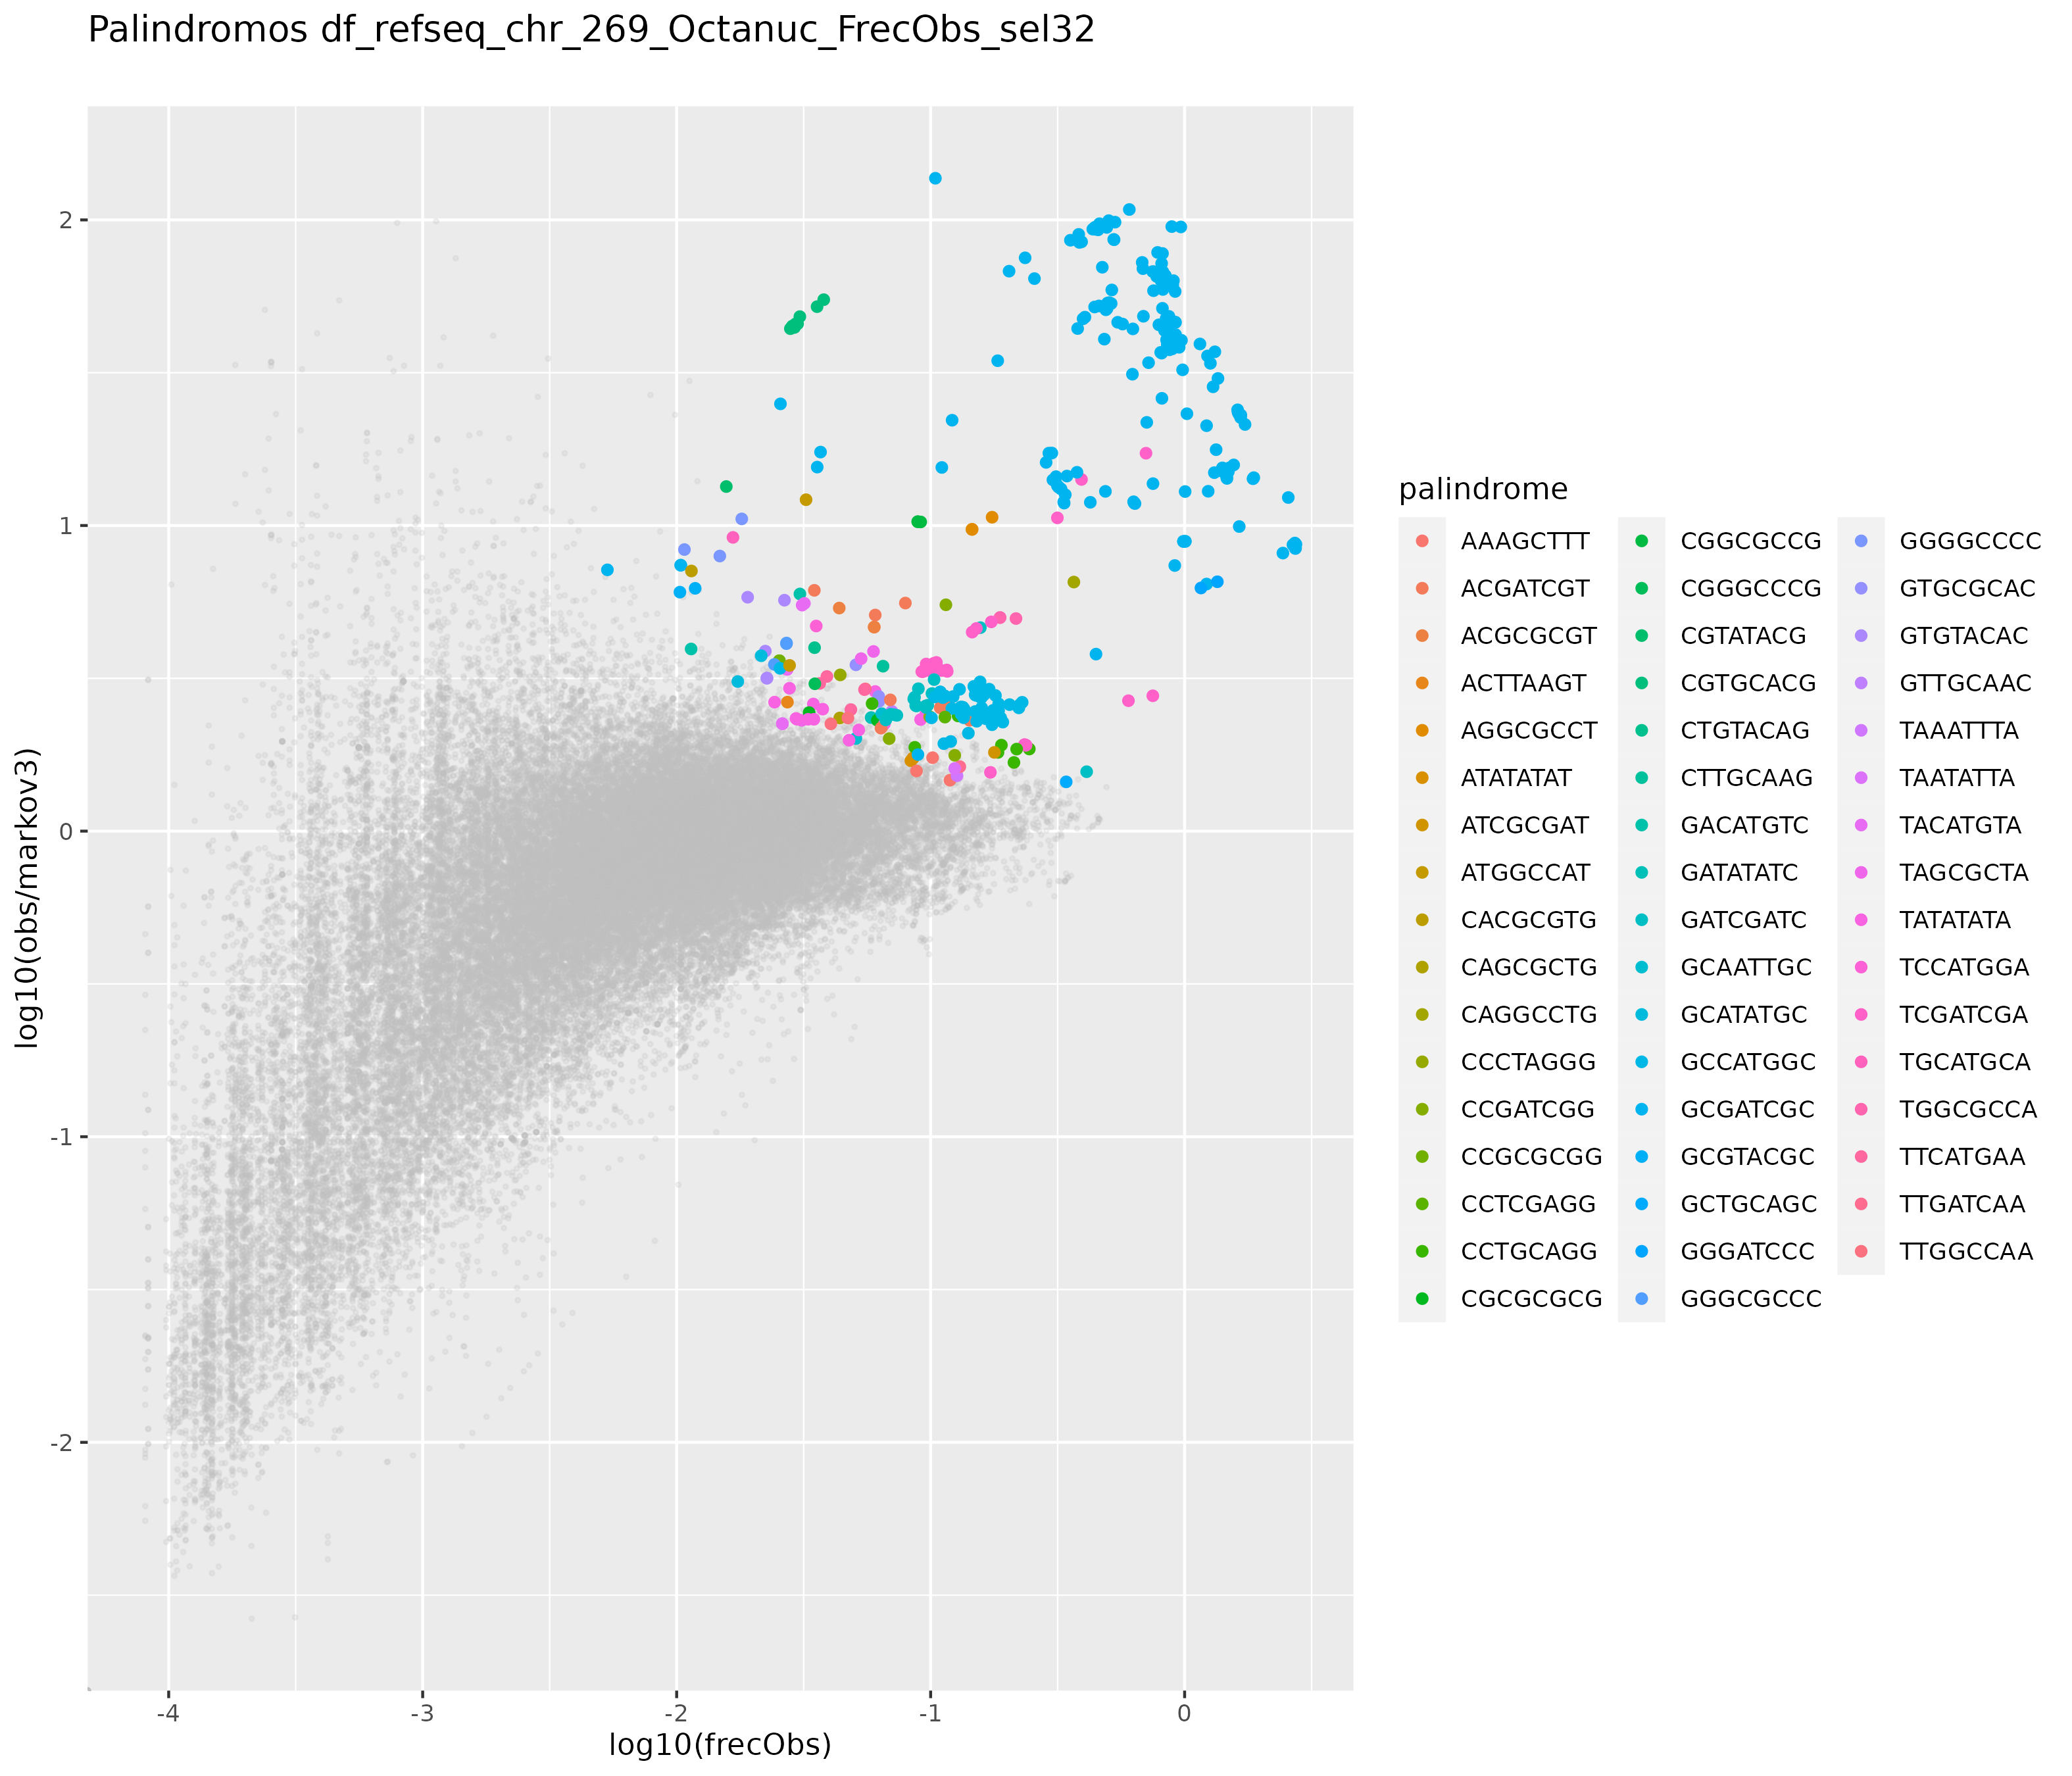
\includegraphics[width=0.8\linewidth]{../PIPELINES_2023/REPORTES/Octanucs_FrecObs/df_refseq_chr_269_Octanuc_FrecObs_sel32_significative-palindromes} 

}

\caption{Here is a nice figure!}\label{fig:nice-fig}
\end{figure}

  \bibliography{book.bib,packages.bib}

\end{document}
